\section{Theoretische Grundlagen}
\label{theorie}



Im Folgenden soll die Bewegungsgleichung für das Pendel hergeleitet werden. Vereinfachend angenommen werden hierzu: Reibungsfreiheit, kleine Auslenkungen sowie die Approximierbarkeit der Masse $m$ durch einen Massepunkt. 
Ausgangspunkt ist hierzu die Erhaltung der Systemenergie $E$, welche sich aufgrund der Annahmen aus potentieller Energie $V$ und kinetischer Energie $T$ zusammensetzt. Es gilt:
\begin{align}
E=T+V=\textrm{const.}
\label{energie}
\end{align}

Des Weiteren gilt für die kinetische Energie $T$, da sich der Massepunkt auf einer Kreisbahn bewegt, dass sich  die relevante Geschwindigkeit $v$ über den Kreisradius bzw. die Länge zwischen Aufhängung und Schwerpunkt $l$ sowie die Winkelgeschwindigkeit $\dot{\varphi}$ darstellen lässt. Mit $v=l\dot{\varphi}$ folgt:
 
\begin{align}
T&=\frac{ml^2\dot{\varphi}^2}{2}
\label{kin}
\end{align}


\begin{figure}
	\centering
	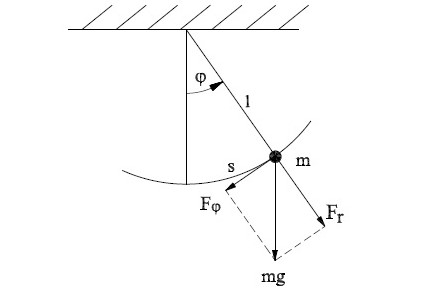
\includegraphics{faden}
	\caption{Die Abbildung zeigt schematisch den Aufbau des Fadenpendels sowie die relevanten Kräfte.}
	\label{faden}
\end{figure}

Aus der Skizze des Fadenpendels \footnote{Skizze entnommen aus dem Informationsmaterial zu den Experimentellen Übungen der Universität Münster 2017, url: https://sso.uni-muenster.de/LearnWeb/learnweb2/pluginfile.php/1334529/mod\_resource/content/1/Fadenpendel\_Einf.pdf }  lesen wir für die potentielle Energie ab:
\begin{align}
V&=-l \cos (\varphi) m g
\label{pot}
\end{align}
Durch Einsetzten von den Gleichungen \cref{kin} und \cref{pot} in Gleichung \cref{energie} erhalten wir:
\begin{align}
E&=-l \cos (\varphi) m g +\frac{ml^2\dot{\varphi}^2}{2}=\textrm{const.}
\end{align}
Dieses lässt sich durch differenzieren nach der Zeit \cref{dt} sowie der Kleinwinkelnäherung und elementaren Umformungen auf die gewünschte Form \cref{diffgl} bringen:
\begin{align}
	0&=lmg \dot{\varphi}\sin (\varphi) +ml^2 \dot{\varphi} \ddot{\varphi}
	\label{dt} \\
	0&=\ddot{\varphi}+\frac{g}{l} \varphi
	\label{diffgl}
\end{align}
Diese lineare Differenzialgleichung zweiter Ordnung lässt sich mit einem komplexwertigen Potenzreihenansatz lösen. Dieser führt mit $\omega:=\sqrt{\frac{g}{l}}$ auf eine Funktion der Form: 
\begin{align}
\varphi(t)=a \sin (\omega t + \varphi_0)
\end{align}
Wobei $a$ und $\varphi_0$ an die Anfangsbedingungen angepasst werden müssen.\\
Eine Pendelschwingung entspricht genau einer Periode($2\pi$) des Sinus. Daher gilt bezüglich der Schwingungsdauer $T$:
\begin{align}
	2\pi = \sqrt{\frac{g}{l}} T \\
	\Leftrightarrow T= 2 \pi \sqrt{\frac{l}{g}}
\end{align}

Es folgt für die Fallbeschleunigung:
\begin{align}
g=\frac{2 \pi l}{T^2}
\label{bestg}
\end{align}\\



Aus Gleichung \ref{bestg} lassen sich zwei Variablen ablesen, welche zu messen sind und deren Unsicherheiten berücksichtigt werden müssen. Die kombinierte Standardunsicherheit setzt sich aus den Unsicherheiten der Länge $l$ und der Schwingungsdauer $T$ zusammen. Da Länge und Zeit in diesem Experiment unabhängige Größen sind, gilt nach GUM:
\begin{align}
u(g)&=\sqrt{\left(\frac{\partial g}{\partial l} u(l)\right)^2 + \left(\frac{\partial g}{\partial T}u(T)\right)^2 } \\
   &= g \sqrt{\left(\frac{u(l)}{l}\right)^2+ \left(2 \frac{ u(T)}{T}\right)^2 }
   \label{kombu}
\end{align}  





